\documentclass[12pt,a4paper,spanish]{article}
\usepackage[a4paper,margin=15mm]{geometry}
\usepackage[utf8]{inputenc}
\usepackage{graphicx}
\usepackage{subcaption}
\usepackage{float}
\usepackage[export]{adjustbox}
\usepackage[spanish]{babel}
\usepackage{url}
%Configuración autores y afiliaciones
\usepackage{authblk}
\renewcommand\Authands{ \& }
\renewcommand{\Affilfont}{\fontsize{9}{12} \selectfont \itshape}
\renewcommand{\Authfont}{\fontsize{12}{14} \selectfont}

%configuración header y foot
\usepackage{fancyhdr}
% http://linorg.usp.br/CTAN/macros/latex/contrib/fancyhdr/fancyhdr.pdf
% check the link above for use guide
\fancyhf{}
\setlength\headheight{40pt}
\setlength\headsep{12pt}
\setlength\voffset{5pt}
\setlength\footskip{11pt}
\renewcommand{\headrulewidth}{1pt}
\fancyhead[L]{Análisis de Datos \\ Científicos con R}
\fancyhead[C]{Informe Final\\ Merenda L.A.}
\fancyhead[R]{
\includegraphics[width=50mm]{fcen_logo.png}}
\renewcommand{\footrulewidth}{1pt}
\fancyfoot[R]{\thepage}
\pagestyle{plain}

\title{Comportamiento eyectivo de una región activa de larga duración: análisis con R}
\author[1]{Merenda, L.A.}
%\author[1,2]{Cremades, H.}
%\author[1,2]{Iglesias, F.A.}
%\author[3,4]{Mandrini, C.H.}
%\author[5]{López, F. M.}
%\author[3]{López-Fuentes, M.C.}

\affil[1]{Facultad de Ciencias Exactas y Naturales. Universidad Nacional de Cuyo}
%\affil[1]{Universidad Tecnológica Nacional, Facultad Regional Mendoza, CEDS, Mendoza, Argentina.}
%\affil[2]{Consejo Nacional de Investigaciones Científicas y Tecnológicas (CONICET), Argentina.}
%\affil[3]{Instituto de Astronomía y Física del Espacio, IAFE (UBA-CONICET), Buenos Aires, Argentina.}
%\affil[4]{Facultad de Ciencias Exactas y Naturales (UBA), Buenos Aires, Argentina.}
%\affil[5]{Instituto de Ciencias Astronómicas, de la Tierra y del Espacio (ICATE), CONICET-UNSJ, San Juan, Argentina.}

% remove vert space taken by date & date isn't printed
\date{\vspace{-5ex}} 

\begin{document}
\maketitle
\pagestyle{fancy}
\thispagestyle{fancy}


\renewcommand{\abstract}{Resumen}
\Resumen{\textbf{Resumen}. Durante 2010 una región activa de larga duración emergió y persistió a lo largo de 5 meses desde julio hasta noviembre. La posición en cuadratura de las naves STEREO permitió el seguimiento continuo de la región e identificación de las eyecciones coronales de masa (ECM) originadas en esta. Investigamos las condiciones que dieron lugar a periodos específicos de de actividad eyectiva en esta región activa, usando datos del instrumento STEREO-SECCHI así como también de los instrumentos AIA y HMI a bordo del Solar Dynamics Observatory. Determinamos las posiciones del origen de las ECM y medimos ancho angular, velocidad y masas de las eyecciones. EL comportamiento de la región durante su pasaje por el frente del disco solar, se analizó siguiendo la distribución espacial y evolución de la densidad de corriente, helicidad de corriente, y otros parámetros extraídos de los datos HMI-SHARP. La búsqueda de correlaciones entre los parámetros fotosféricos de la región y los períodos de intensa actividad eyectiva es alentadora para poder entender los mecanismos físicos en juego y así mejorar los modelos de meteorología espacial.}

\vspace{8ex}

\section{Introducción}
 Las Eyecciones Coronales de Masa (ECM), suponen un alto peligro para los sistemas tecnológicos espaciales y terrestres, son los principales moduladores del clima espacial. Si bien se han propuestos diferentes mecanismos que dan lugar a una ECM, aún no hay consenso sobre cual es el principal y por lo tanto los pronósticos actuales no logran predecir donde y cuándo tendrá lugar la próxima erupción.
 Las regiones activas (RA) solares son sitios de campos magnéticos intensos, generalmente complejos y altamente dinámicos. Dentro de las regiones activas, emergen tubos de flujo magnético luego de haber atravesado la zona de convección, y se revelan en la fotósfera como regiones de polaridad magnética opuesta, cuya complejidad puede crecer debido a diversos movimientos fotosféricos. Estos desplazamientos arrastran las bases de las líneas de campo magnético, creando campos magnéticos coronales de gran tensión, a la vez que se inyecta continuamente flujo en la corona. La energía magnética se acumula gradualmente en un estado de cuasi-equilibrio, hasta que se libera por algún mecanismo disparador, resultando frecuentemente en una ECM. Si bien las regiones activas son reconocidas como una fuente común de ECMs, poco se conoce acerca de que circunstancias hacen que una región activa (RA) particular sea la siguiente en originar una ECM, o cuando en el tiempo esta eyección tendrá lugar. Dado el potencial de las ECMs de desencadenar tormentas geomagnéticas, se hace urgentemente necesario encontrar respuestas a estos problemas.

\newpage

\subsection{La región activa en estudio}
La RA seleccionada, que persistió hasta 5 rotaciones, apareció por primera vez en el limbo este como la región activa 11089 (designación de la NOAA), el 19 de julio de 2010. Para ese entonces, las naves gemelas STEREO estaban aproximándose a una posición de cuadratura con respecto a la tierra, esto es, logrando una separación de $180^{\circ}$ entre ambas naves. Al mismo tiempo, la misión SDO estaba comenzando su fase operacional, y proveyó las mejores observaciones de la región activa mientras esta transitaba el lado frontal del sol. Si bien el estudio de la región en su totalidad también abarcó tanto el análisis e identificación de cada eyección mediante la confección de animaciones de imágenes del  sol en el extremo ultravioleta (193 \AA) obtenidos de los instrumentos SECCHI abordo de STEREO y AIA abordo de SDO, en el presente informe nos vamos a concentrar en el análisis de datos fotosféricos de la RA.

\section{Búsqueda de datos}
Antes del análisis fotosférico, hubo un trabajo previo de descarga, procesado de datos y confección de animaciones para el período de 5 rotaciones que duró la RA, mediante los cuales se identificaron 108 erupciones del tipo ECM originadas en la región, de este total quedaron un total de 36 que caen en el período de datos fotosféricos. A su vez, estas erupciones están caracterizadas en base a cantidades morfológicas y/o dinámicas las cuales son : ancho angular, ángulo de posición central, masa, velocidad lineal, energía potencial y energía cinética.\par 
Para el análisis de parámetros fotosféricos de la RA se determinaron +-4 días desde que la región activa se encontraba en el centro del disco solar, lo que nos da un total de 9 días para cada región. Para estos intervalos de tiempo mostrados en el cuadro \ref{tabla:1}, optamos por los datos "SHARP" generados en el Joint Science Operation Center (JSOC) mediante el procesado de datos "crudos" del instrumento Helioseismic Magnetic Imager (HMI) abordo del observatorio Solar Dynamics Observatory (SDO). Estos datos consisten en varios "segmentos" los cuales pueden ser mapas espaciales de campo magnético, o Dopplergrams, etc. Junto con estos, vienen los parámetros computados para la región entera de nuestro interés. Cabe aclarar que estos datos pueden venir o no, a nuestra elección, mapeados a una proyección cilíndrica de igual área, siendo esta última la utilizada. Cada segmento es un recorte de la imagen total del sol correspondiente a la región identificada con un número.\par

\begin{table}[h!]
\begin{center}
\begin{tabular}{ |c|c|c|c|c| } 
 \hline
  HARP & NOAA & Fecha comienzo & Meridiano-central & Fecha-final \\
 \hline
  92 & 11089 & 21/07/10 & 25/07/10 & 28/07/10 \\ 
  \hline
 135 & 11100 & 18/08/10 & 22/08/10 & 25/08/10 \\ 
  \hline
 175 & 11106 & 13/09/10 & 17/09/10 & 20/09/10 \\ 
 \hline
 211 & 11112 & 10/10/10 & 14/10/10 & 17/10/10 \\
 \hline
 245 & 11121 & 07/11/10 & 11/11/11 & 14/11/10 \\
 \hline
\end{tabular}
\caption{Intervalos de tiempo de datos descargados para las 5 rotaciones. En la primer y segunda columna, se muestran los números de identificación de la RA. Tercer, cuarta y quinta columna corresponden a las fecha inicial, en meridiano central, y final respectivamente}
\label{tabla:1}
\end{center}
\end{table}

Los parámetros en los que estamos interesados son el flujo magnético total, densidad de corriente promedio, helicidad de corriente promedio, total y valor absoluto total. El interés viene dado que varios estudios han encontrado cierta correlación entre estas cantidades y los períodos eruptivos de una región activa. Estos parámetros ya vienen computados para el recorte de la región entera, pero a nosotros nos interesa estudiar la variación local respecto de cada erupción, por lo que se calcularon para cada erupción estos parámetros en recortes cuadrados de 30x30 píxeles y 90x90 píxeles centrados en el origen de cada evento.\par
\newpage
Cabe señalar aquí que el procesamiento de todos los datos y el computo de los parámetros se hizo en IDL (Interactive Data Language), ya que es el lenguaje mundialmente utilizado por la comunidad de física solar y para la cual esta disponible para cualquier persona la familia de librerías "SolarSoft". Los Datos finales a analizar con herramientas de R son series de tiempo de estos 5 parámetros fotosféricos para cada uno de estas 36 erupciones que se muestran señaladas en la figura \ref{fig:figura1}.

\begin{figure}[h!]
    \centering    
    \begin{subfigure}{.5\textwidth}
    \centering
    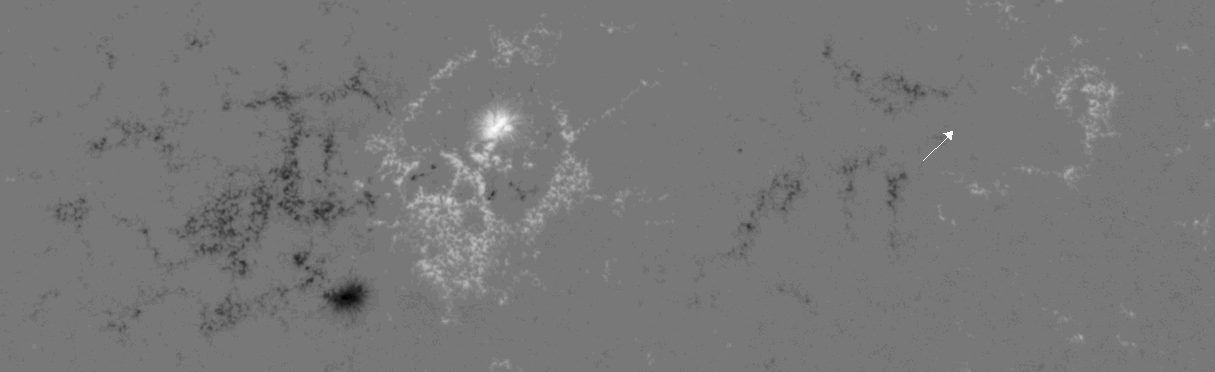
\includegraphics[width=.8\linewidth,scale=0.8]{Br+maskal_92_events.png}
    \caption{1a}
    \label{fig:sfig11}
    \end{subfigure}%
    \begin{subfigure}{.5\textwidth}
    \centering
    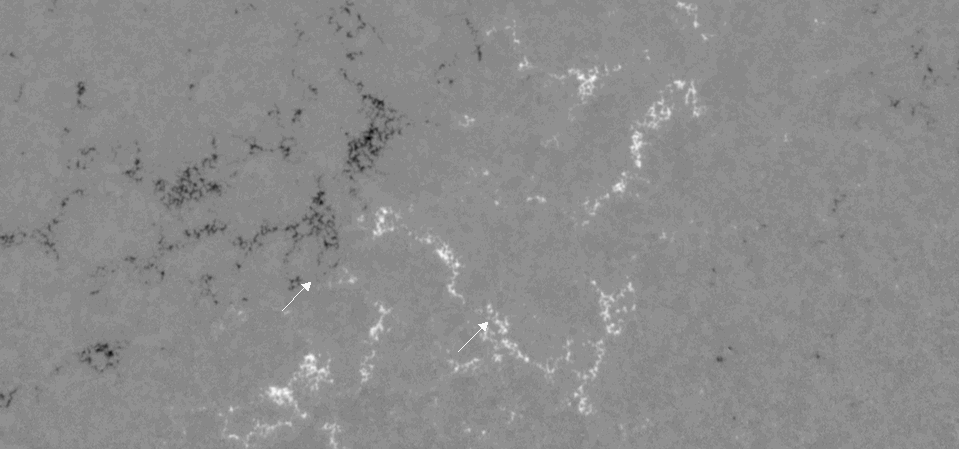
\includegraphics[width=.8\linewidth,scale=0.8]{Br+maskal_135_events.png}
    \caption{1b}
    \label{fig:sfig12}
    \end{subfigure}
    \begin{subfigure}{.5\textwidth}
    \centering
    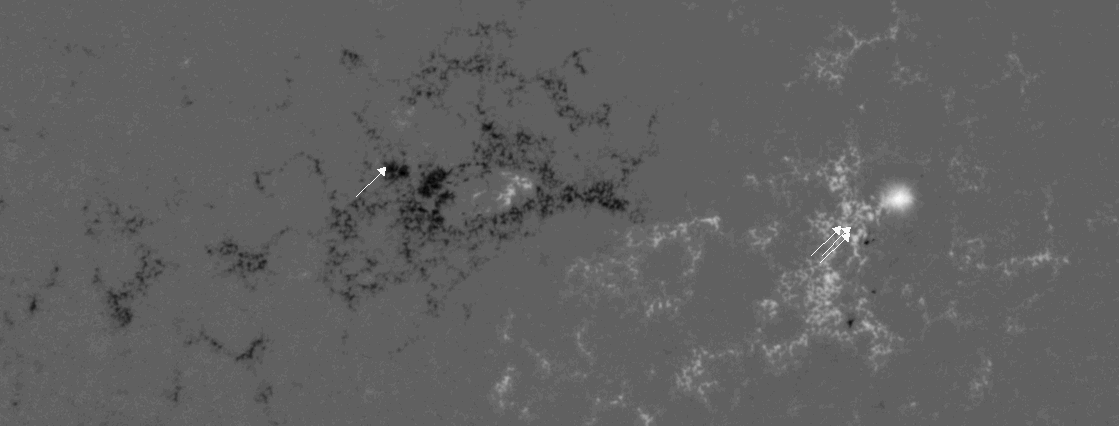
\includegraphics[width=.8\linewidth,scale=0.8]{Br+maskal_175_events.png}
    \caption{1c}
    \label{fig:sfig13}
    \end{subfigure}%
    \begin{subfigure}{.5\textwidth}
    \centering
    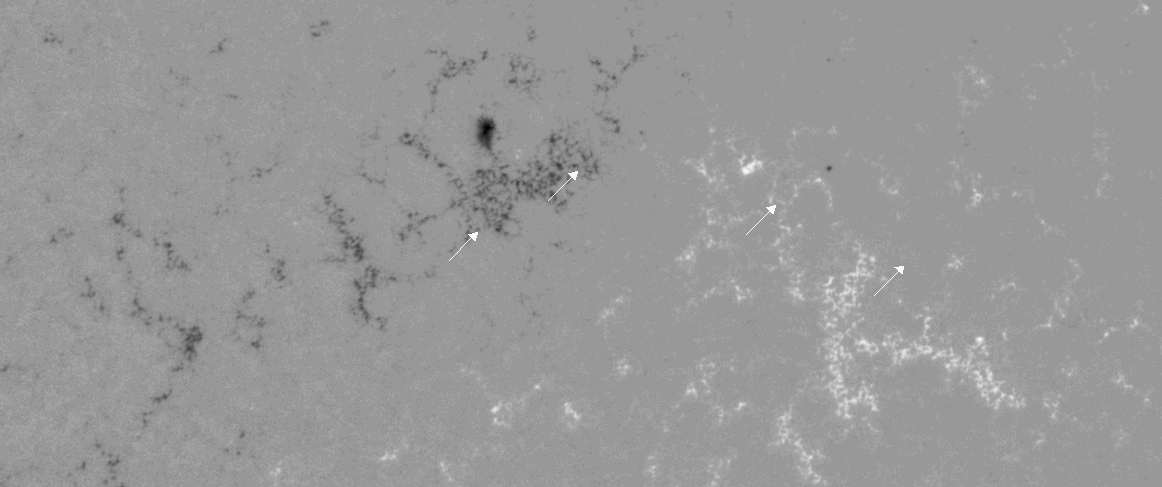
\includegraphics[width=.8\linewidth,scale=0.8]{Br+maskal_211_events.png}
    \caption{1d}
    \label{fig:sfig14}
    \end{subfigure}
    \begin{subfigure}{.5\textwidth}
    \centering
    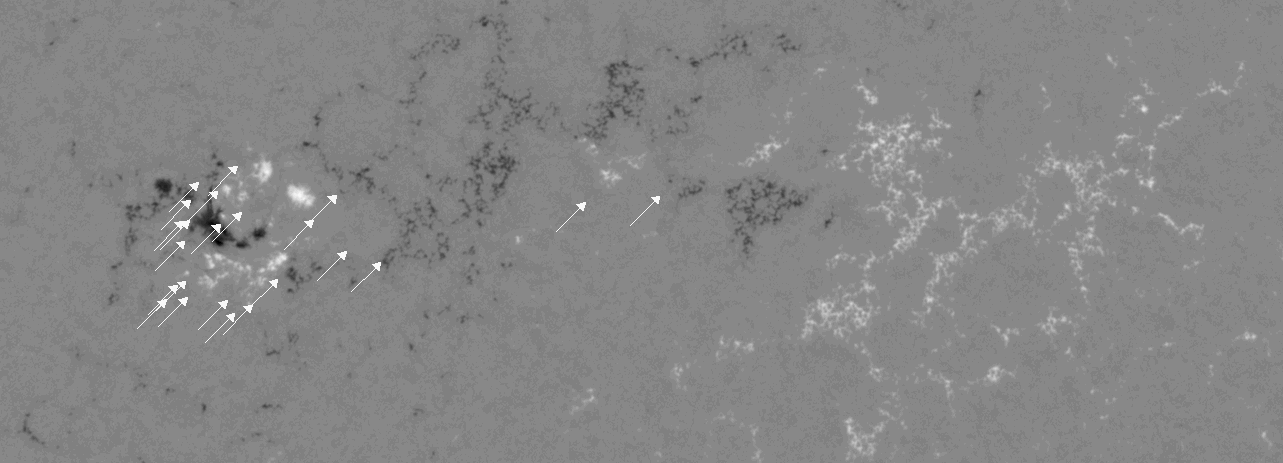
\includegraphics[width=.8\linewidth,scale=0.8]{Br+maskal_245_events.png}
    \caption{1e}
    \label{fig:sfig15}
    \end{subfigure}
    \caption{Región en estudio para las 5 rotaciones con origen de erupciones marcados. Las figuras \ref{fig:sfig11} a \ref{fig:sfig15} corresponden a la región en estudio para fechas de meridiano central en el mismo orden de la \ref{tabla:1}. Cada flecha blanca indice el origen de una erupción, totalizando 36 para las 5 rotaciones. }
    \label{fig:figura1}
\end{figure}

\newpage
\section{Análisis con herramientas de R y resultados}
A partir de los datos previamente generados con IDL y "Solarsoft", se estudió cuales serían las mejores maneras de analizar esta enorme cantidad de datos haciendo uso del lenguaje R. La primer decisión fue solo analizar por el momento las series de tiempo correspondientes a los recortes de 30x30 píxeles. 
La primer manera de visualizar estos datos fue utilizando las librerías "ggplot2", "dplyr" y "lubridate", para normalizar las series de tiempo de cada evento a la hora día de la erupción y graficar para cada parámetro la evolución de las 36 series de tiempo, con la esperanza de observar algún patrón o comportamiento similar previo a la erupción que sugiera un análisis más exhaustivo, en la figura \ref{fig:figura2} se muestran los "plots" obtenidos. Como se logra observar, a simple vista no encontramos nada que se distinga o llame la atención.

\begin{figure}[H]
    \centering
    \begin{subfigure}{.5\textwidth}
    \centering
    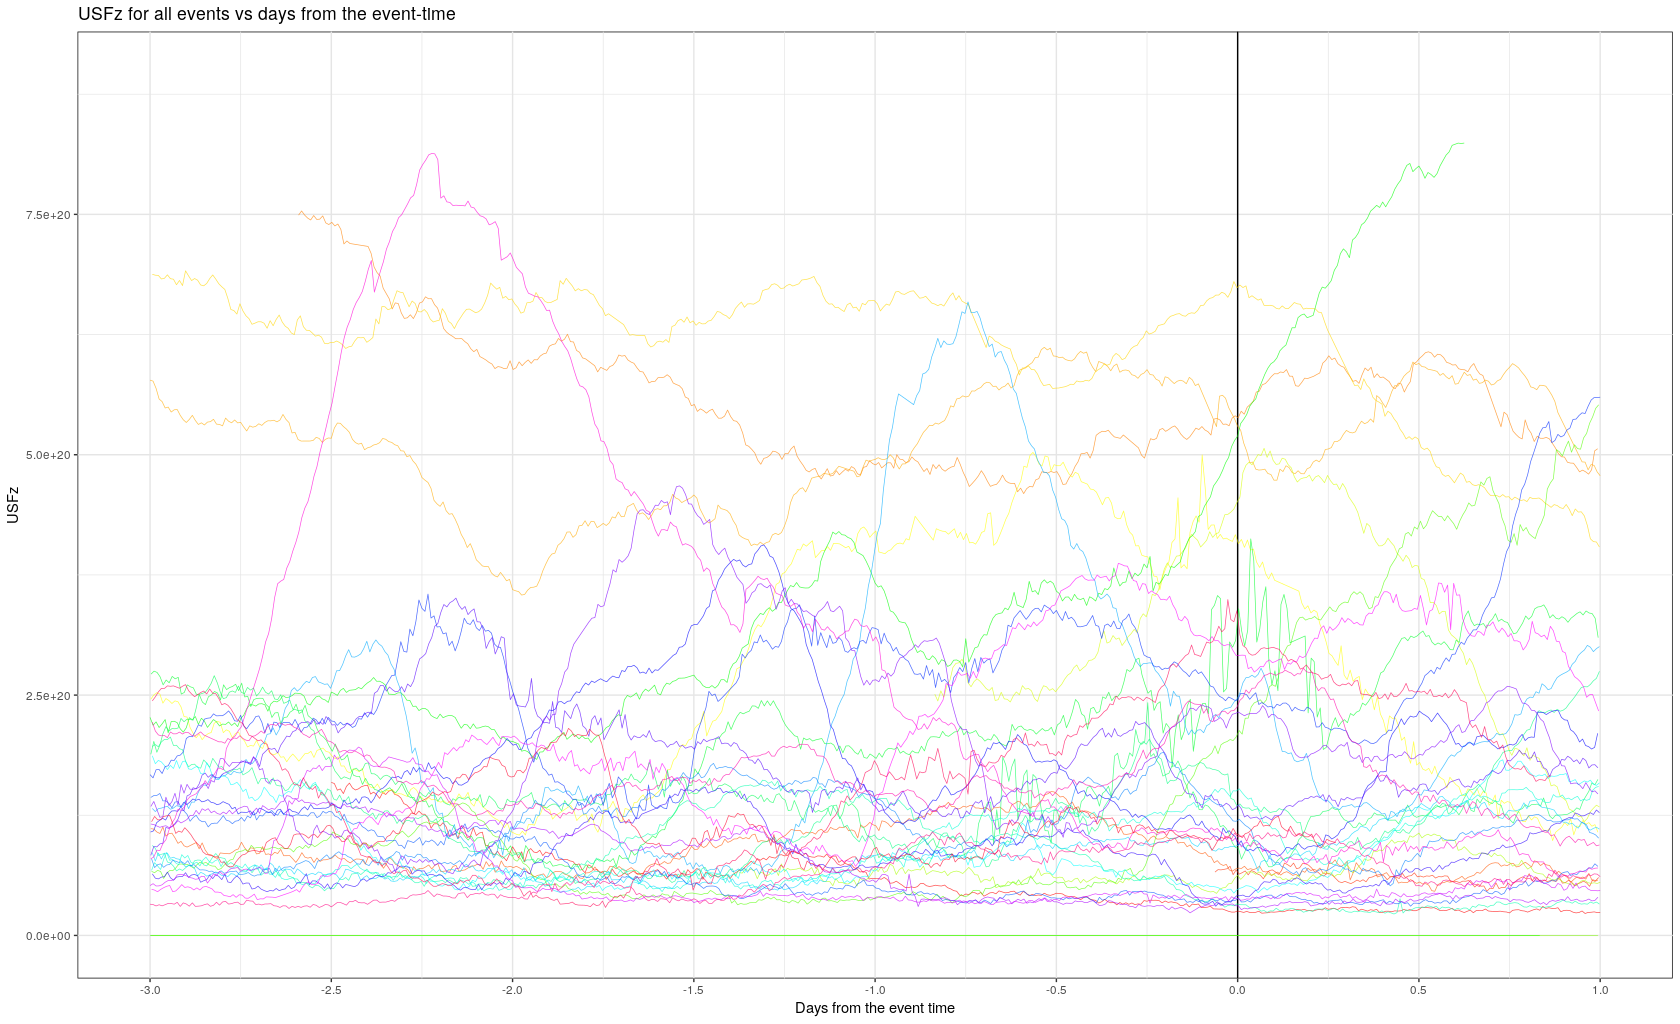
\includegraphics[width=.8\linewidth,scale=0.5]{Rplot.png}
    \caption{2a}
    \label{fig:sfig21}
    \end{subfigure}%
    \begin{subfigure}{.5\textwidth}
    \centering
    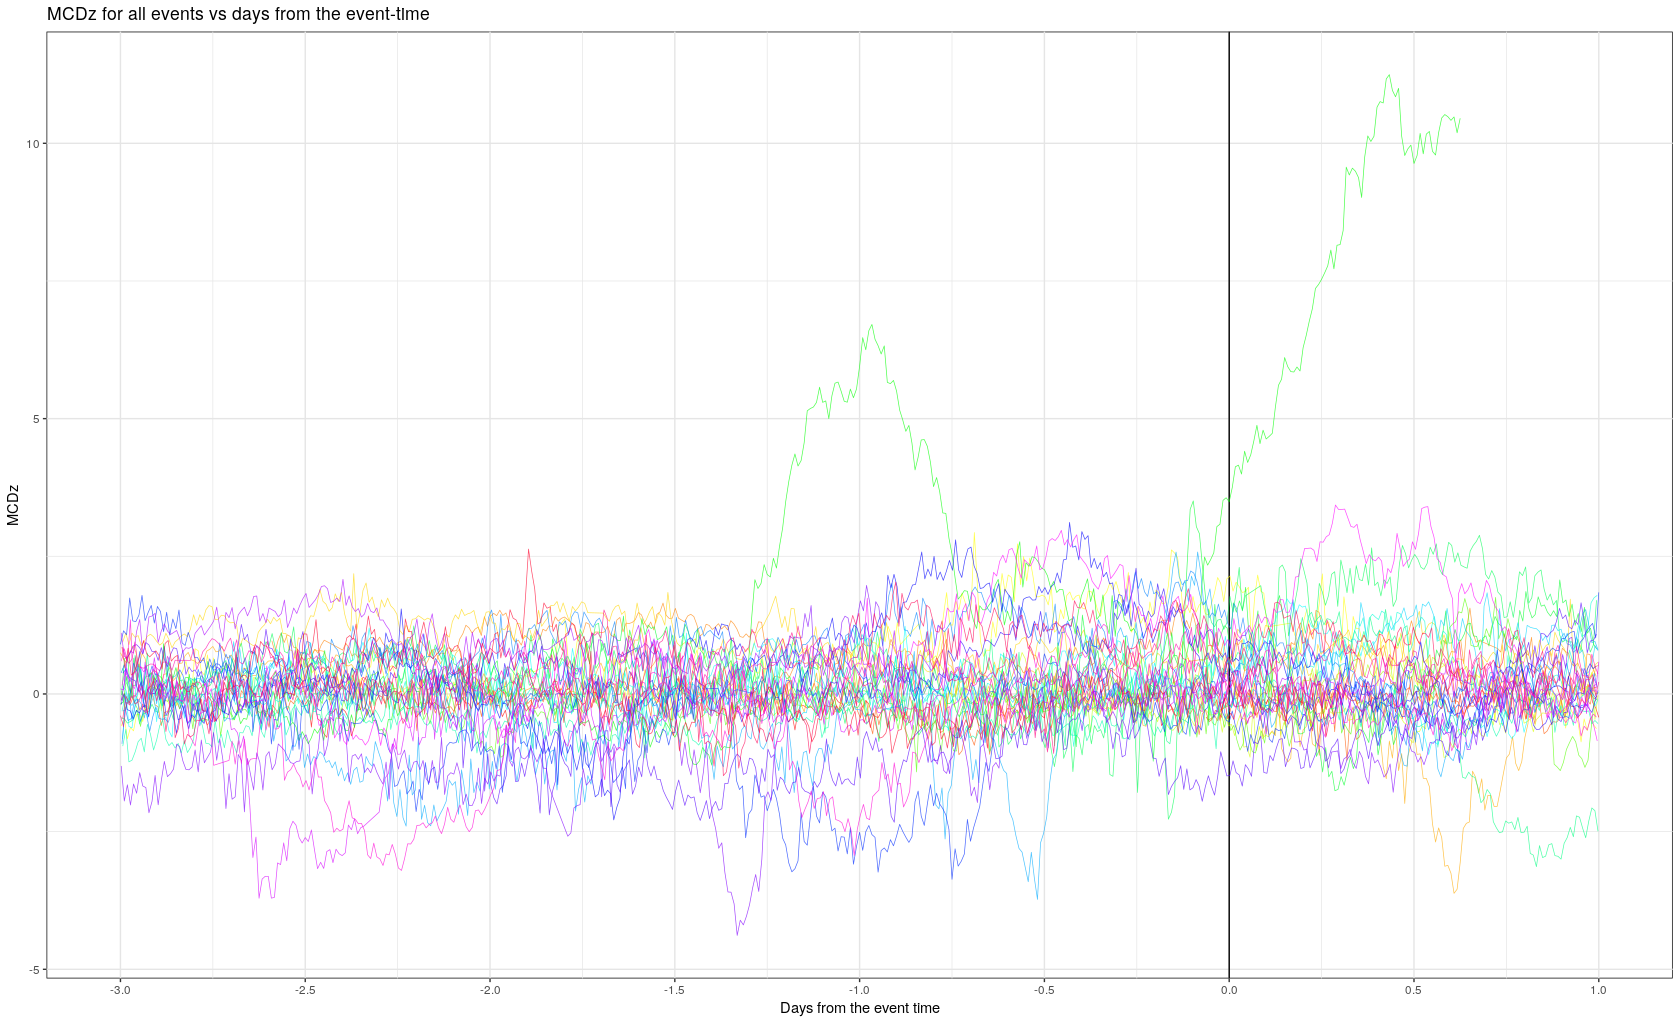
\includegraphics[width=.8\linewidth,scale=0.5]{Rplot01.png}
    \caption{2b}
    \label{fig:sfig22}
    \end{subfigure}
    \begin{subfigure}{.5\textwidth}
    \centering
    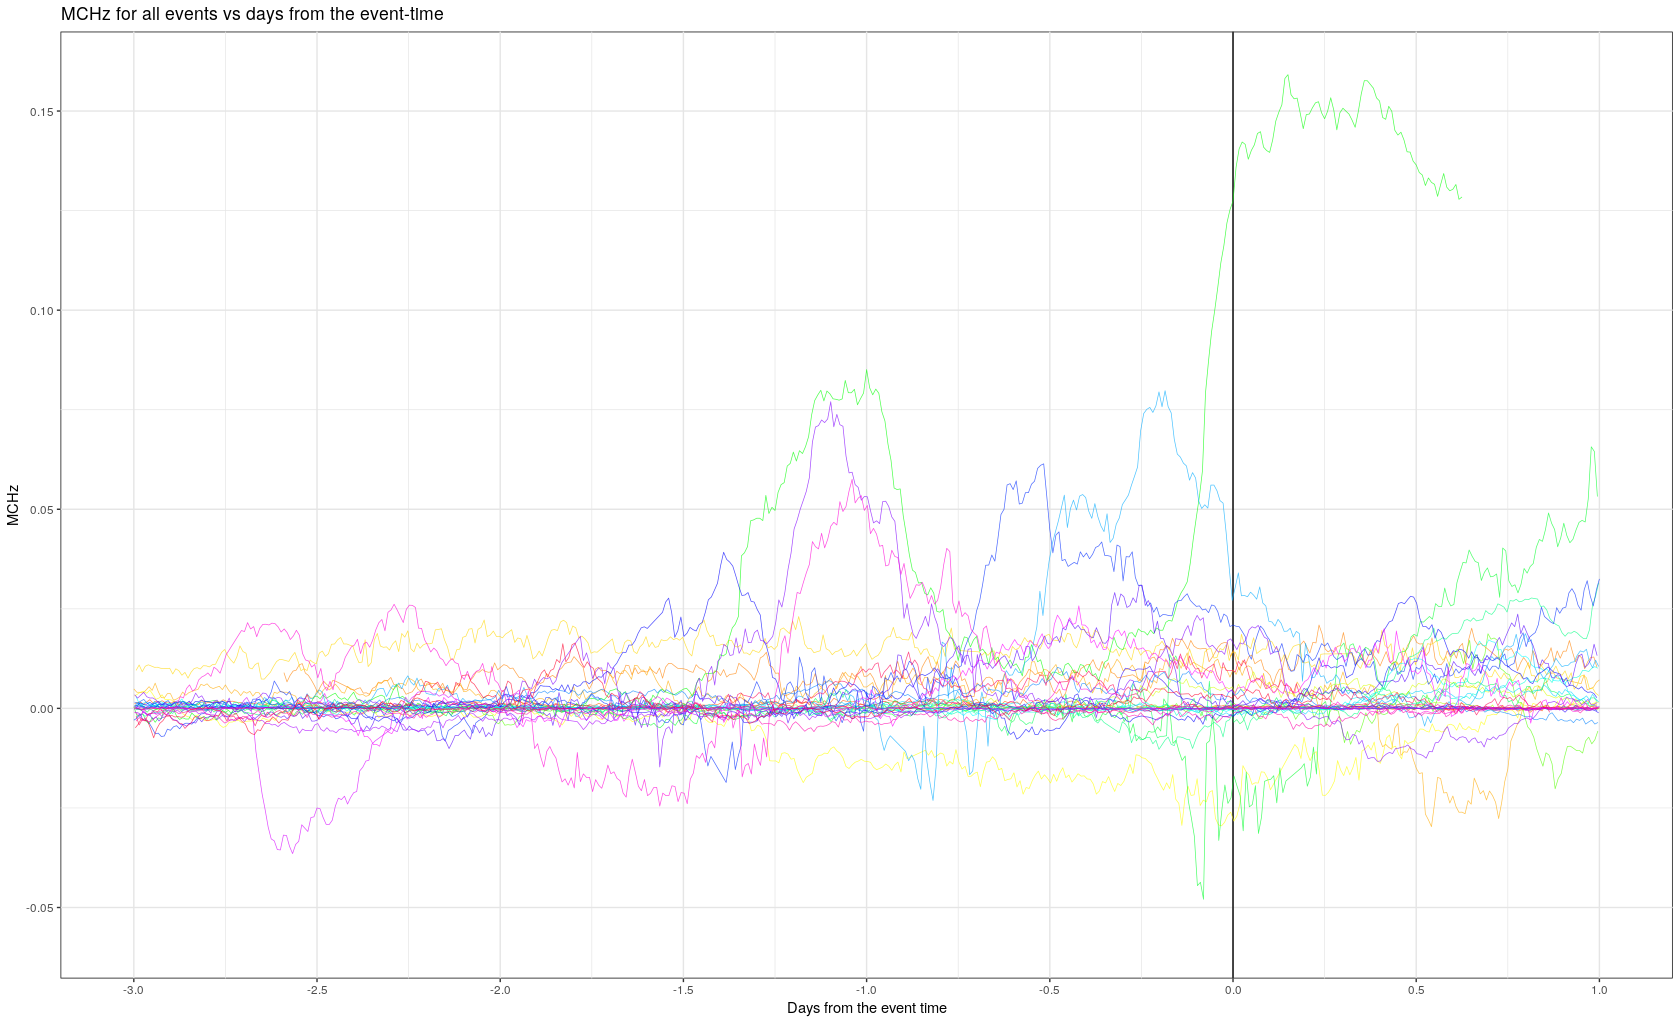
\includegraphics[width=.8\linewidth,scale=0.5]{Rplot02.png}
    \caption{2c}
    \label{fig:sfig23}
    \end{subfigure}%
    \begin{subfigure}{.5\textwidth}
    \centering
    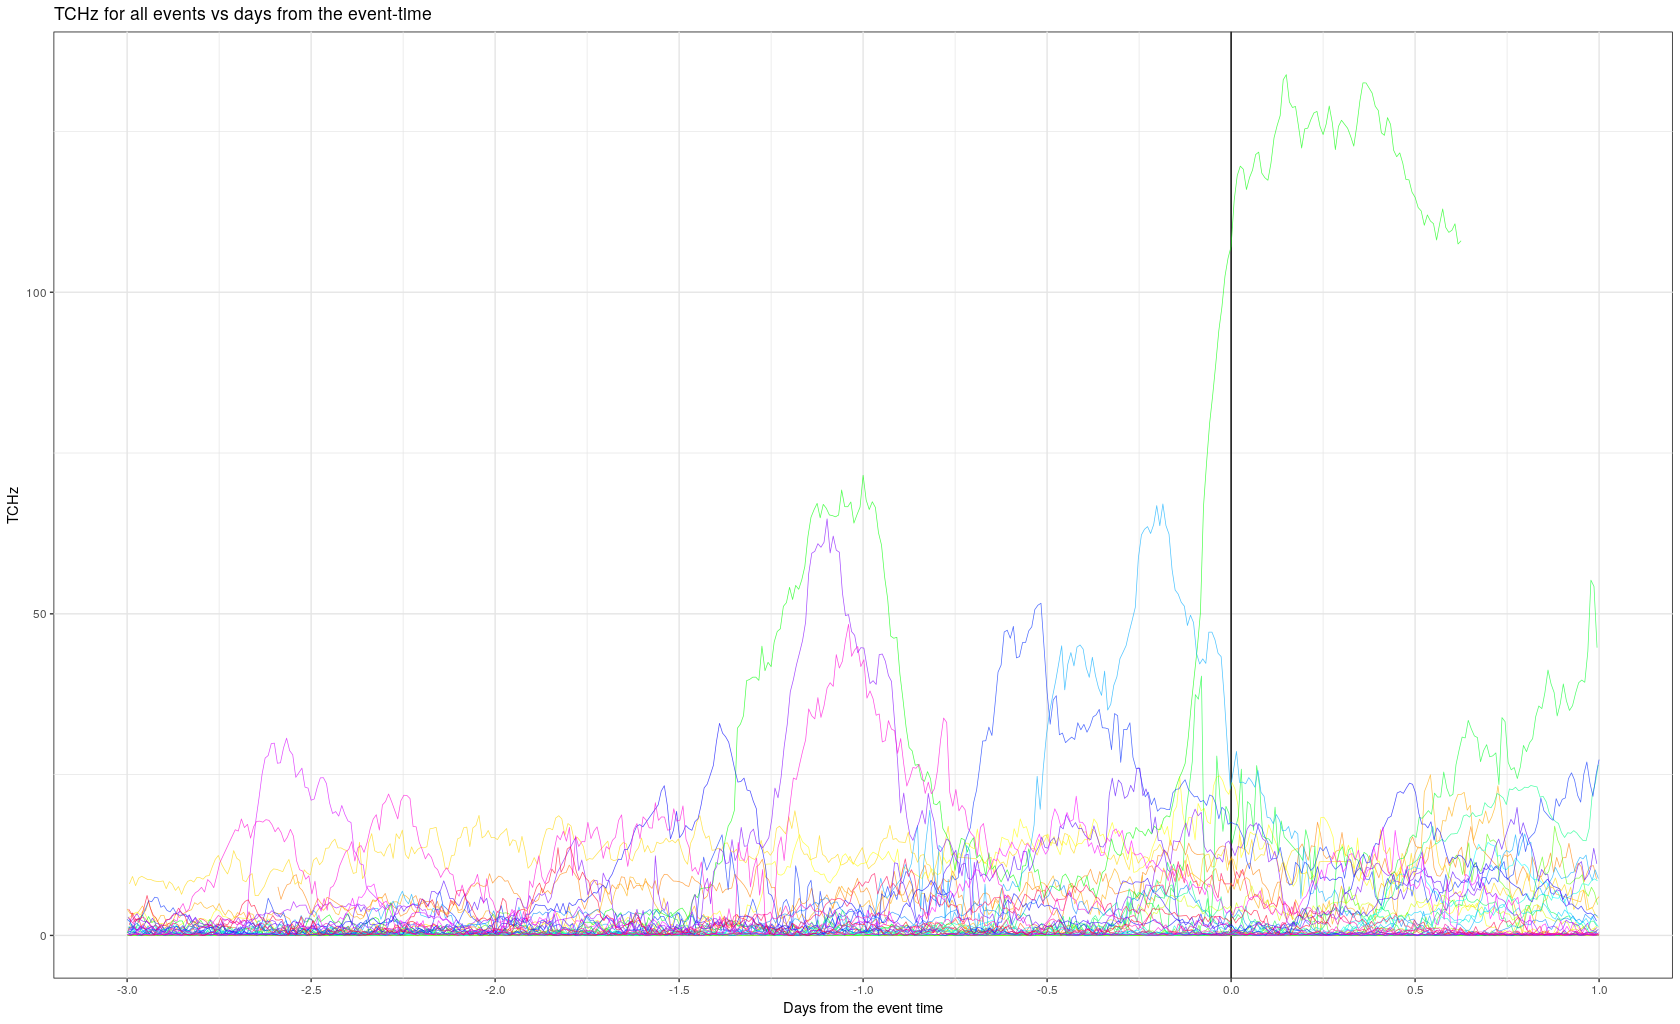
\includegraphics[width=.8\linewidth,scale=0.5]{Rplot03.png}
    \caption{2d}
    \label{fig:sfig24}
    \end{subfigure}
    \caption{Gráficas de parámetros fotósfericos computados para 36 recortes correspondientes a cada erupción. Figura \ref{fig:sfig21} corresponde a "usfz", \ref{fig:sfig22} a "mcdz", \ref{fig:sfig23} a "mchz" y \ref{fig:sfig24} a "tchz".}
    \label{fig:figura2}
\end{figure}

Luego procedimos a intentar encontrar que tan bien correlacionan los valores de características morfológicas y/o dinámicas con los valores de parámetros fotósfericos en el momento de la erupción o en momentos anteriores de la erupción en un intervalo de tiempo establecido. Para este caso debimos explorar las librerías disponibles en el CRAN para el análisis de series de tiempo. Hay muchas librerías destinadas para este fin "forecast","ggTimeSeries","TSstudio","sugrrants","tsbox", entre muchas otras. Si bien son de alta utilidad se decidió por simplicidad y homogeneidad manipular solo listas, vectores, data-frames y/o tibbles. De las herramientas que ofrecen estas librerías solo se usó la función ts\_lag() del paquete "tsbox", que es un conjunto de funciones agnósticas a los tipos de datos que le damos.\par
Para primero encontrar las Correlaciones, de los datos originales importados de archivos csv, creamos series de tiempo para cada parámetro particular ya sea fotósferico o morfológico/dinámico. Luego desarrollé 3 funciones auxiliares:
\begin{itemize}
  \item "snum2str": para traducir tiempo en segundos del tipo númerico en strings. Esta función se hizo para poder utilizar ts\_lag generando los intervalos de tiempo numericamente, y luego traducirlo a strings.
  \item "swp\_mp": toma como argumentos:un intervalo de tiempo dado, la lista de series de tiempo de algún parámetro fotosférico, y la serie de tiempo de los eventos seleccionados de alguna de sus características morfológicas y/o dinámicas, con los cuales calcula la regresión lineal, factor de correlación y el tibble con los datos utilizados correspondientes al intervalo de tiempo ingresado.
  \item "sw\_md" : extiende la funcionalidad de "swp\_mp" a n intervalos de tiempo tomando como argumentos los mismos que "swp\_mp".
\end{itemize}

Aquí la función que nos permite obtener el dato final a analizar es "sw\_md", que aplica en n intervalos de tiempo "swp\_mp" a las series de tiempo. Definimos un vector de intervalos de tiempo de 1 hora desde el momento de la erupción hasta 3 días atrás. Lo que nos da un total de 73 intervalos de tiempo. Ahora bien podríamos en principio aplicar la función a cualquier combinación posible de parámetros disponibles, pero tenemos:\\
\textbullet \hspace{1ex}5 fotosféricos 
\begin{itemize}
    \item usfz (Suma total de Flujo Magnético sin signo)
    \item mcdz (Densidad de corriente promedio)
    \item mchz (Helicidad de corriente promedio)
    \item absnchz (Valor absoluto neto de la helicidad de corriente)
    \item tchz (Suma total de Helicidad de corriente sin signo)
\end{itemize}
\noindent
\textbullet \hspace{1ex}6 Morfológicos/dinámicos
\begin{itemize}
    \item angwid (Ancho angular de la erupción)
    \item cpa (Ángulo de posición central)
    \item lisp (Velocidad lineal)
    \item poe (Energía potencial)
    \item kie (Energía cinética)
\end{itemize}

Si quisiéramos analizar todas las posibles combinaciones tendríamos un total de 30, cada una con 73 regresiones lineales, 73 data-frames de datos y 30 data-frames de la evolución del factor de correlación respecto del intervalo de tiempo. Para este informe solo se analizaron las siguientes combinaciones:
\begin{itemize}
    \item usfz vs angwid
    \item usfz vs kie
    \item tchz vs angwid
    \item tchz vs kie
\end{itemize}

En la figura \ref{fig:figura3} se grafican el valor del factor de correlación r en función del intervalo t en horas para las 4 combinaciones de parámetros seleccionadas.

\begin{figure}[h!]
    \centering
    \begin{subfigure}{.5\textwidth}
    \centering
    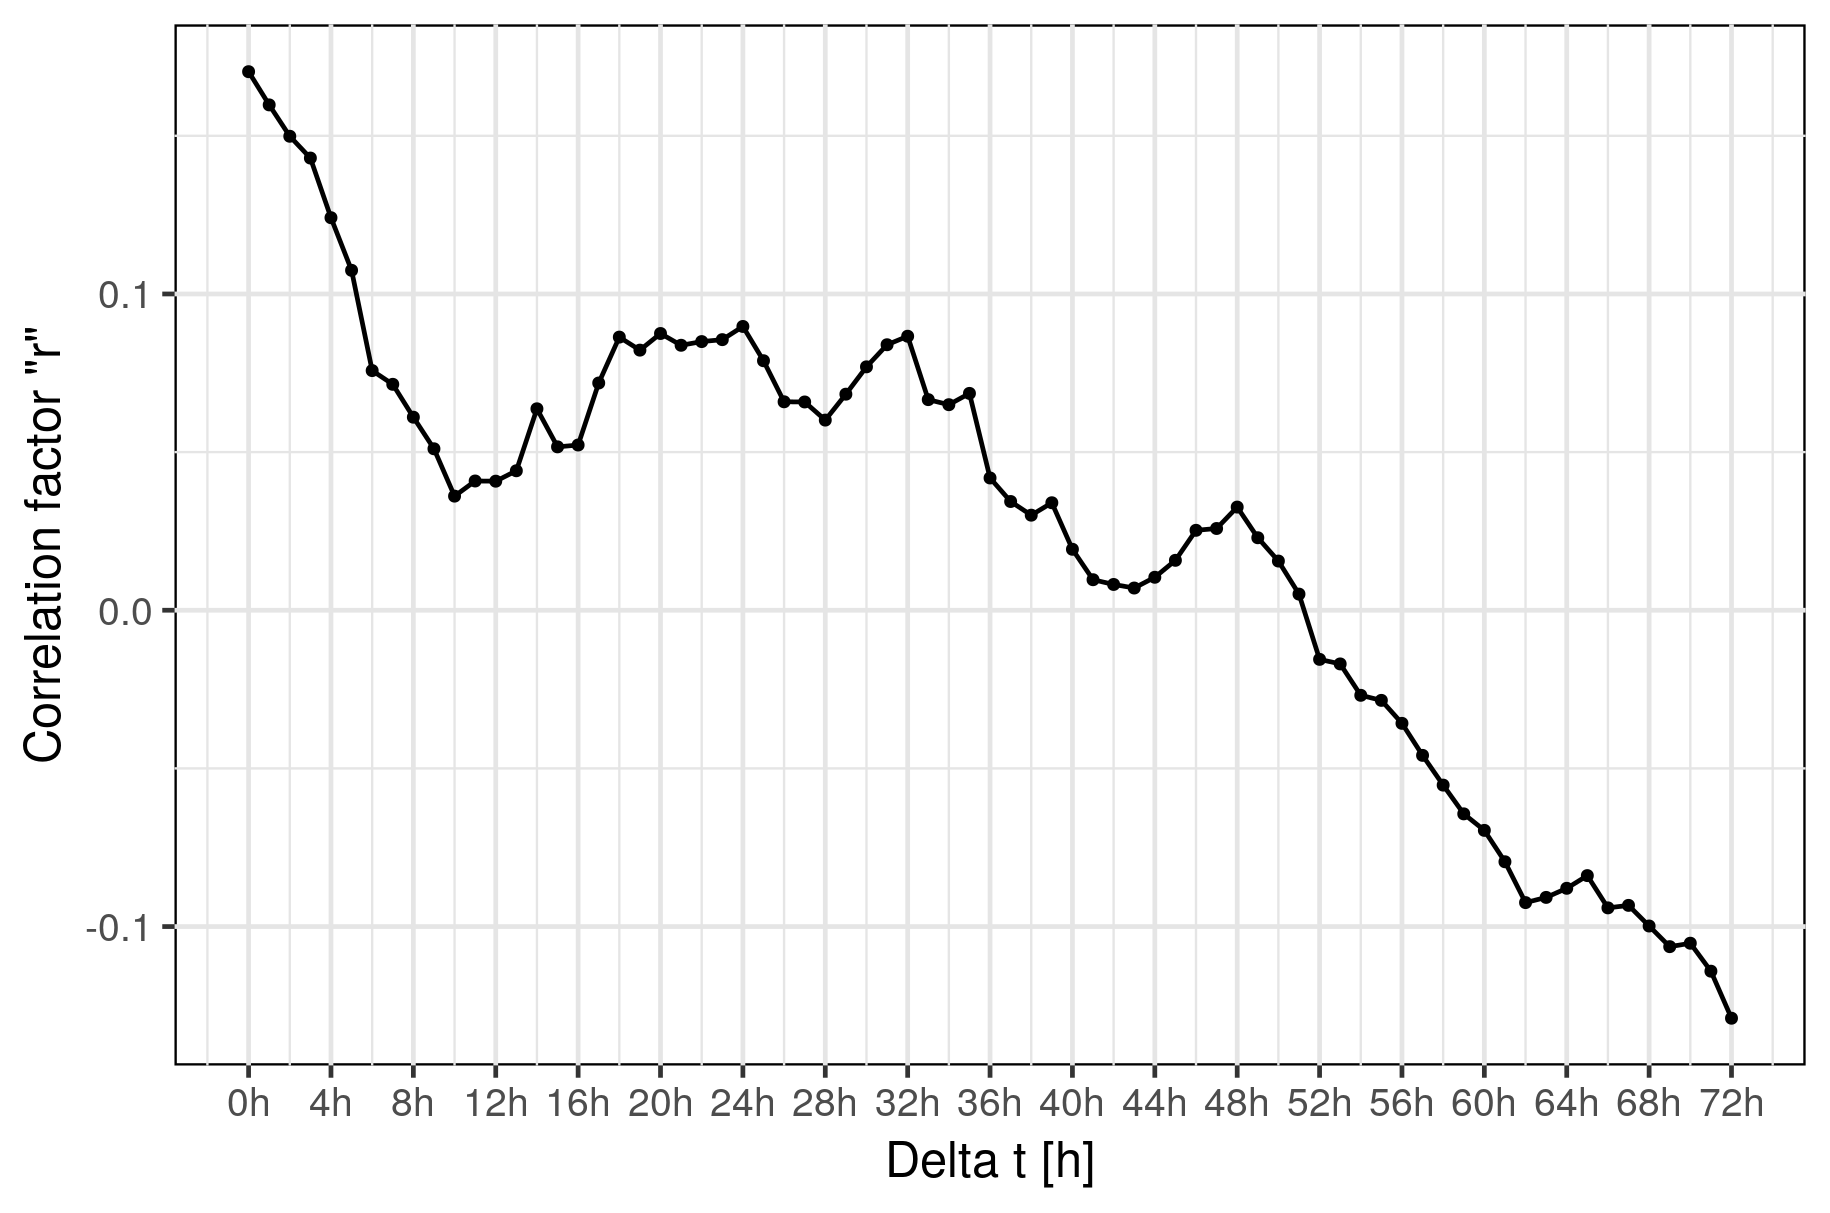
\includegraphics[width=.8\linewidth,scale=0.8]{usfzangwid_corfac.png}
    \caption{3a}
    \label{fig:sfig31}
    \end{subfigure}%
    \begin{subfigure}{.5\textwidth}
    \centering
    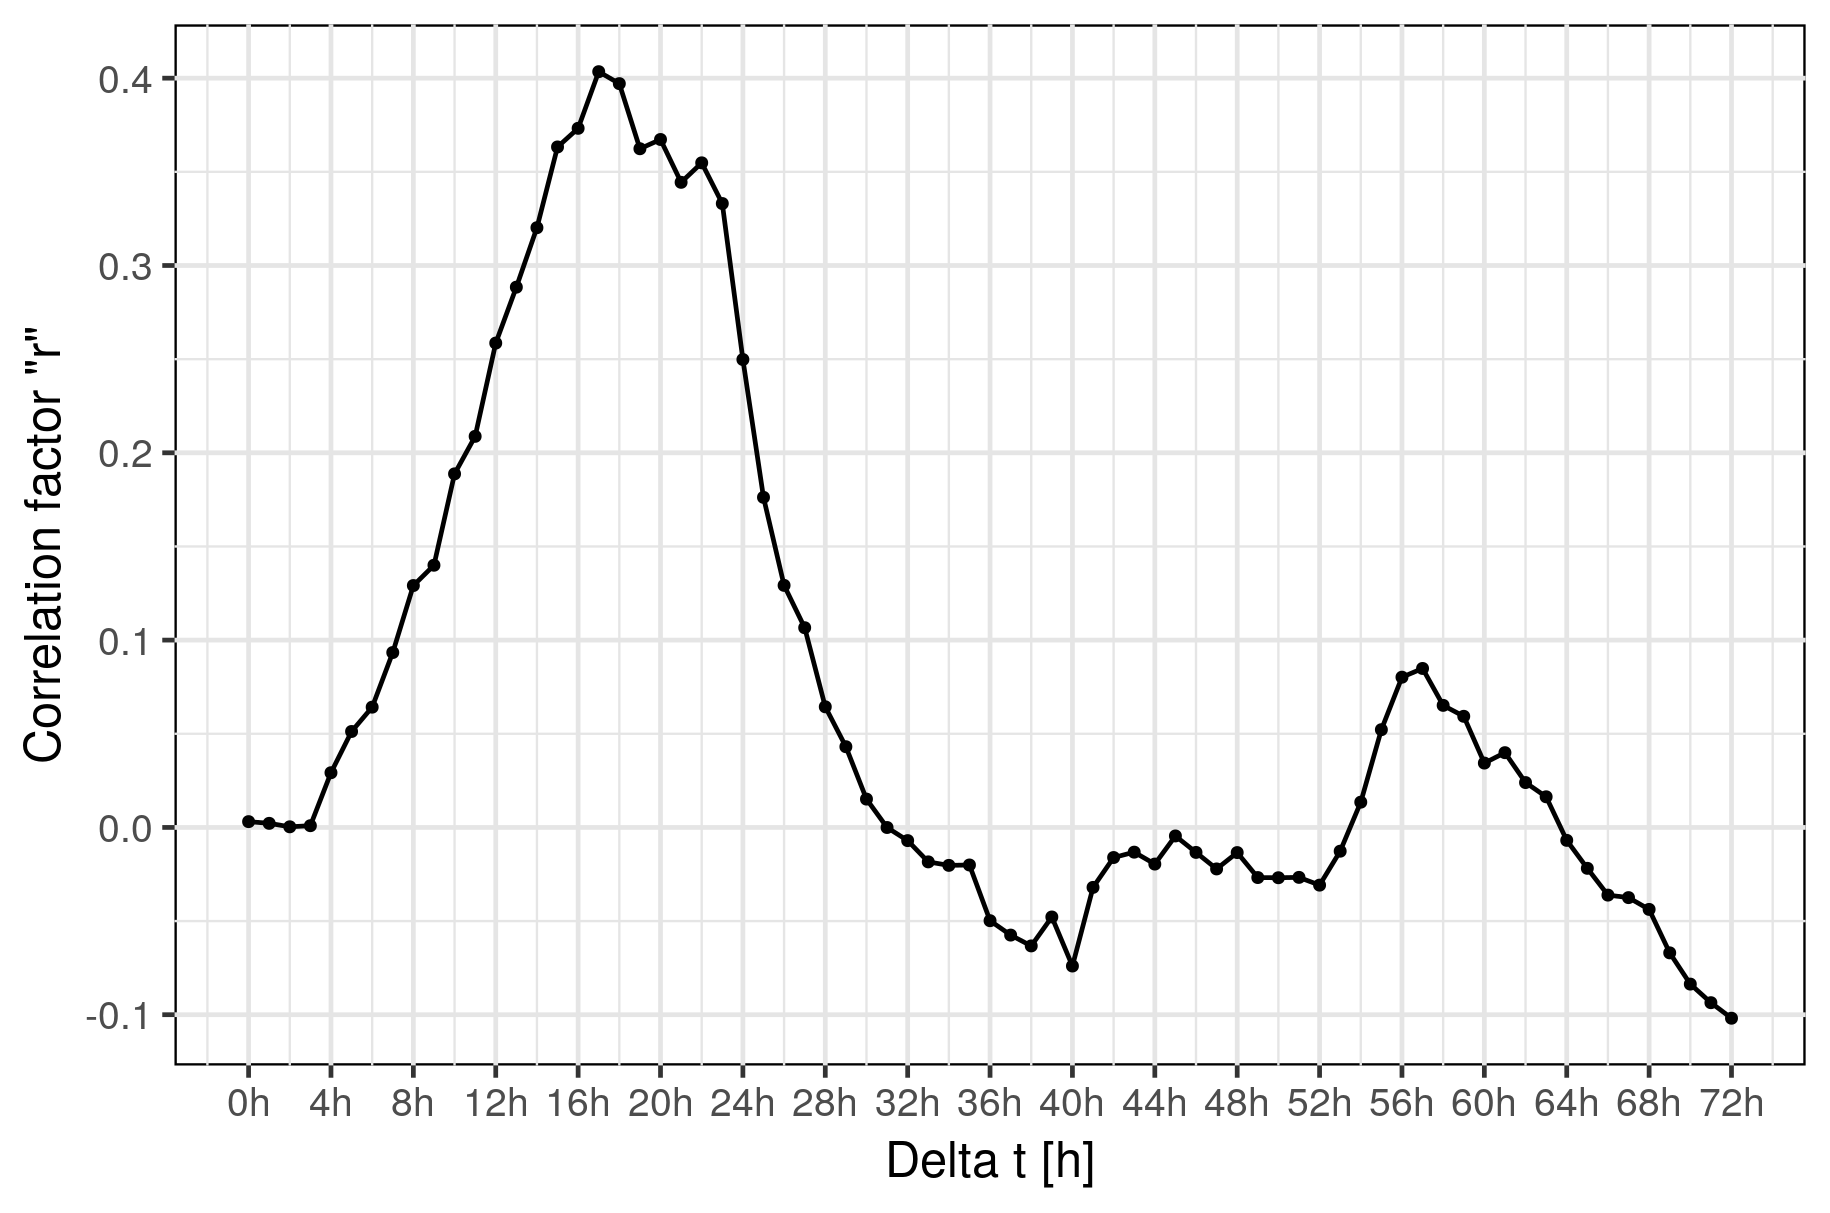
\includegraphics[width=.8\linewidth,scale=0.8]{usfzkie_corfac.png}
    \caption{3b}
    \label{fig:sfig32}
    \end{subfigure}
    \begin{subfigure}{.5\textwidth}
    \centering
    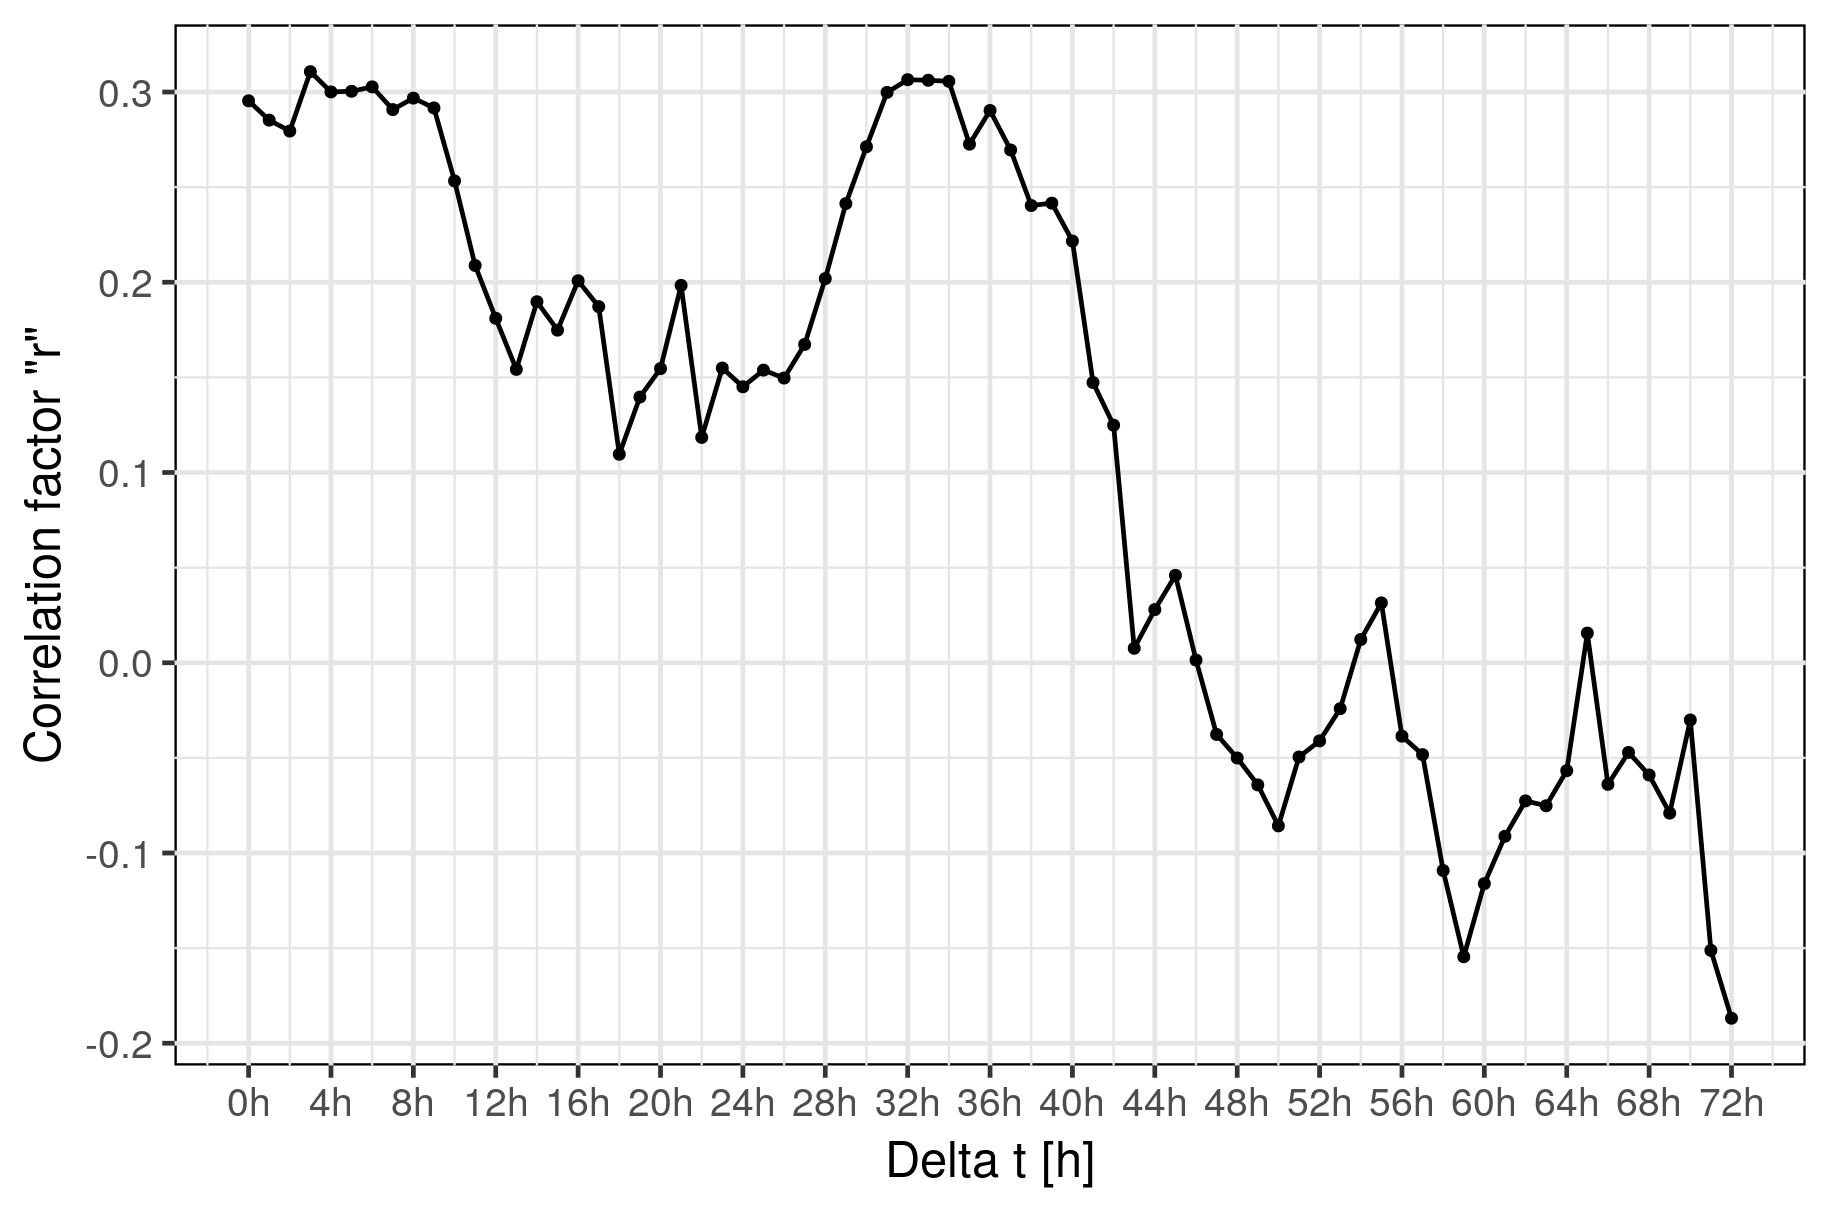
\includegraphics[width=.8\linewidth,scale=0.8]{tchzangwid_corfac.png}
    \caption{3c}
    \label{fig:sfig33}
    \end{subfigure}%
    \begin{subfigure}{.5\textwidth}
    \centering
    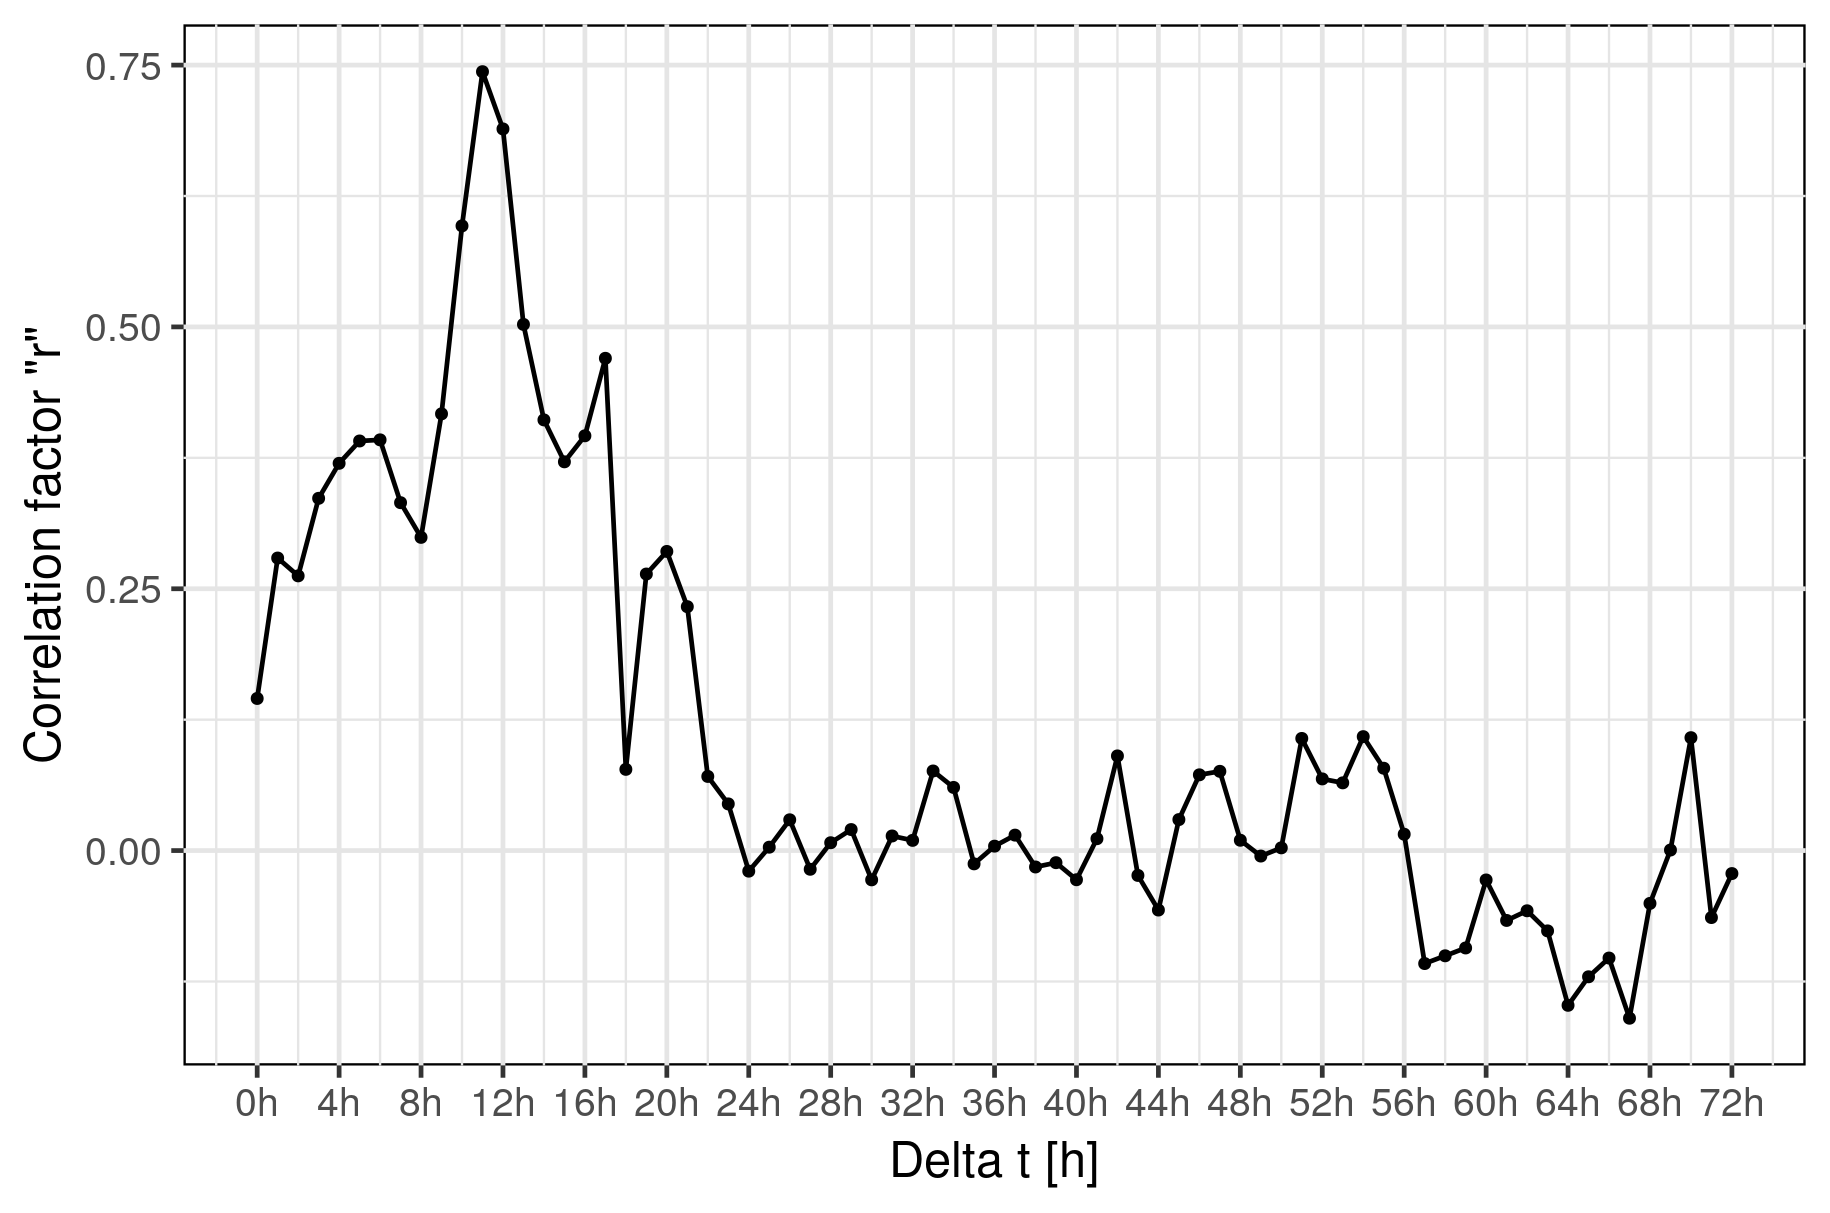
\includegraphics[width=.8\linewidth,scale=0.8]{tchzkie_corfac.png}
    \caption{3d}
    \label{fig:sfig34}
    \end{subfigure}
    \caption{Evolución del factor de correlación en función del intervalo de tiempo.Figura \ref{fig:sfig31} corresponde a " usfz vs angwid", \ref{fig:sfig32} a " usfz vs kie", \ref{fig:sfig33} a "tchz vs angwid " y \ref{fig:sfig34} a "tchz vs kie". }
    \label{fig:figura3}
\end{figure}

\newpage
\section{Conclusiones}
El análisis de estas series de tiempo muestra que no hay buena correlación entre estos parámetros a diferentes intervalos de tiempo, los valores de correlación son muy bajos. De todas maneras, solo corresponde a la combinatoria de 4 series temporales, faltando un total de 26 combinaciones posibles a analizar. \par
Si bien el análisis de series de tiempo en R tiene su propios tipos de objetos y muchas librerías desarrolladas para su manipulación (por ej. "forecast", "ggTimeSeries", "tsbox", entre muchas otras), se optó por manejarlas como si fueran tibbles o data-frames por simplicidad y para no romper con el formato utilizado en el paquete de librerías "tidyverse" del cual se utilizaron el tidyverse-core ("ggplot2","purr","dplyr","tibble","stringr") y otras como "lubridate" para el manejo de fechas y tiempos, "magrittr" para piping.\par
En la búsqueda de librerías que sean de utilidad encontramos a "gganimate" que queda como trabajo a futuro poder animar la evolución de los gráficos de dispersión de cada regresión lineal con cada intervalo de tiempo.

\newpage
\section{Bibliografía}

Wickham H (2016). ggplot2: Elegant Graphics for Data Analysis. Springer-Verlag New York. ISBN 978-3-319-24277-4, http://ggplot2.org. \\

Grolemund G, Wickham H (2011). “Dates and Times Made Easy with lubridate.” Journal of Statistical Software, 40(3), 1–25. http://www.jstatsoft.org/v40/i03/. \\

H. Cremades, C. H. Mandrini, B. Schmieder, A. M. Crescitelli, Coronal Mass Ejections from the Same Active Region Cluster: Two Different Perspectives, Sol. Phys.290 (2015) 1671–1686. arXiv:1505.01384, doi:10.1007/s11207-015-0717-9 \\

Cremades, H., Mandrini, C., Fuentes, M., Merenda, L., Cabello, I., López, F., Poisson, M. (2016). A long-duration active region: Evolution and quadrature observations of ejective events. Proceedings of the International Astronomical Union, 12(S327), 60-66. doi:10.1017/S174392131700028X \\

Cabello, I., Cremades, H., Balmaceda, L. et al. Sol Phys (2016) 291: 1799.\\ https://doi.org/10.1007/s11207-016-0941-y \\

Cremades, H., Bothmer, V.: 2004, On the three-dimensional configuration of coronal mass ejections. Astron. Astrophys. 422, 307.  \\

Bobra, M.G., Sun, X., Hoeksema, J.T. et al. Sol Phys (2014) 289: 3549.\\ https://doi.org/10.1007/s11207-014-0529-3 \\

Hoeksema, J.T., Liu, Y., Hayashi, K. et al. Sol Phys (2014) 289: 3483.\\ https://doi.org/10.1007/s11207-014-0516-8 \\

Couvidat, S., Schou, J., Hoeksema, J.T. et al. Sol Phys (2016) 291: 1887.\\ https://doi.org/10.1007/s11207-016-0957-3 \\

Thompson W. Coordinate systems for solar image data. ASTRON ASTROPHYS. 2006;449 (2):791-803. \\

R. A. Howard, J. D. Moses, A. Vourlidas, J. S. Newmark, D. G. Socker, S. P. Plunkett, C. M. Korendyke, J. W. Cook, A. Hurley, J. M. Davila, et al., Sun Earth Connection Coronal and Heliospheric Investigation (SECCHI), Space Sci. Rev.136 (2008) 67–115. doi:10.1007/s11214-008-9341-4. \\

G. E. Brueckner, R. A. Howard, M. J. Koomen, C. M. Korendyke, D. J. Michels, J. D. Moses, D. G. Socker, K. P. Dere, P. L. Lamy, A. Llebaria, M. V. Bout, R. Schwenn, G. M. Simnett, D. K. Bedford, C. J. Eyles, The Large Angle Spectroscopic Coronagraph (LASCO), Sol. Phys.162 (1995) 357–402.doi:10.1007/BF00733434. \\
J. R. Lemen, A. M. Title, D. J. Akin, P. F. Boerner, C. Chou, J. F. Drake, D. W. Duncan, C. G. Edwards, F. M. Friedlaender, G. F. Heyman, et al., The Atmospheric Imaging Assembly (AIA) on the Solar Dynamics Observatory (SDO), Sol. Phys.275 (2012) 17–40. doi:10.1007/s11207-011-9776-8. \\

P. H. Scherrer, J. Schou, R. I. Bush, A. G. Kosovichev, R. S. Bogart, J. T. Hoeksema, Y. Liu, T. L. Duvall, J. Zhao, A. M. Title, C. J. Schrijver, T. D. Tarbell, S. Tomczyk, The Helioseismic and Magnetic Imager (HMI) Investigation for the Solar Dynamics Observatory (SDO), Sol. Phys.275 (2012) 207–227. doi:10.1007/s11207-011-9834-2. \\

\end{document}
